\chapter{Project Schedule Management}
In this section, we will elaborate on the subsequent activities that followed the development of the initial Gantt chart and Work Breakdown Structure (WBS). We will provide detailed information about the development team members and the milestones that have been established. Finally, we will present the final Gantt chart and the network diagram, illustrating the comprehensive planning and scheduling of the project.


\section{Project Team}
\begin{itemize}
    \item \textbf{Project Manager:} Tony Prince
    \item \textbf{Team Leader:} Karan Goel
    \item \textbf{Business Analyst:} Banin Sensha Shrestha
    \item \textbf{Network Specialist:} Dipesh Baral
    \item \textbf{Programmer/Analyst:} Kushal Rimal
    \item \textbf{Programmer/Analyst:} Affan Mehmood
\end{itemize}

\section{Project Milestones}
\begin{enumerate}
    \item \textbf{Project Kick-Off Milestone:}
    This marks the official start of the project, involving setting up and conducting the kick-off meeting. The agenda is prepared and all team members and stakeholders are notified and encouraged to understand their roles and responsibilities.

    \item \textbf{Budget Approval Milestone:}
    Achieved upon successful estimation and approval of the project budget, encompassing tasks such as budget estimation and securing necessary approvals.
    

    \item \textbf{Planning Phase Completion Milestone:}
    Completion of the planning phase, including integration of data analysis tools, creation of the Work Breakdown Structure (WBS), survey preparation, requirements analysis, risk management planning, budget estimation, and project schedule development. This milestone transitions the project from planning to execution.
    
    \item \textbf{Gantt Chart Creation Milestone:}
    Completion of the project scheduling phase with the creation of the Gantt chart, facilitating visual tracking of project activities and timelines.
    
    \item \textbf{Design Phase Completion Milestone:}
    Completion of the design phase, including the design of user interfaces and back-end systems, approval of Business Process Documents (BPD), and planning for hardware design and integration. This milestone prepares the project for a smooth transition to the development phase.
    
    \item \textbf{Execution Phase Completion Milestone:}
    Represents the end of the execution phase, with major tasks such as the implementation of system components like Recreation Programs Registration, Health-Management Classes Registration, Tracking System, Incentive System, and hardware installation completed.
    
    \item \textbf{Testing and Quality Assurance Milestone:}
    Focuses on ensuring the system's readiness and reliability before deployment, including all levels of testing (unit, integration, user) and resolution of any issues, preparing the system for go-live.
    
    \item \textbf{Monitoring and Promotion Milestone:}
    Beyond project completion, this milestone ensures the ongoing operation and promotion of the system, including system monitoring, addressing operational issues, gathering user feedback for continuous improvement, providing hyper-care support, and promotional activities to boost system usage among employees.
\end{enumerate}

The Recreation and Wellness Intranet project's work breakdown structure with eight milestones is depicted in Figure \ref{fig:gnt3}, and \ref{fig:gnt4} respectively.

\begin{figure}[ht]
    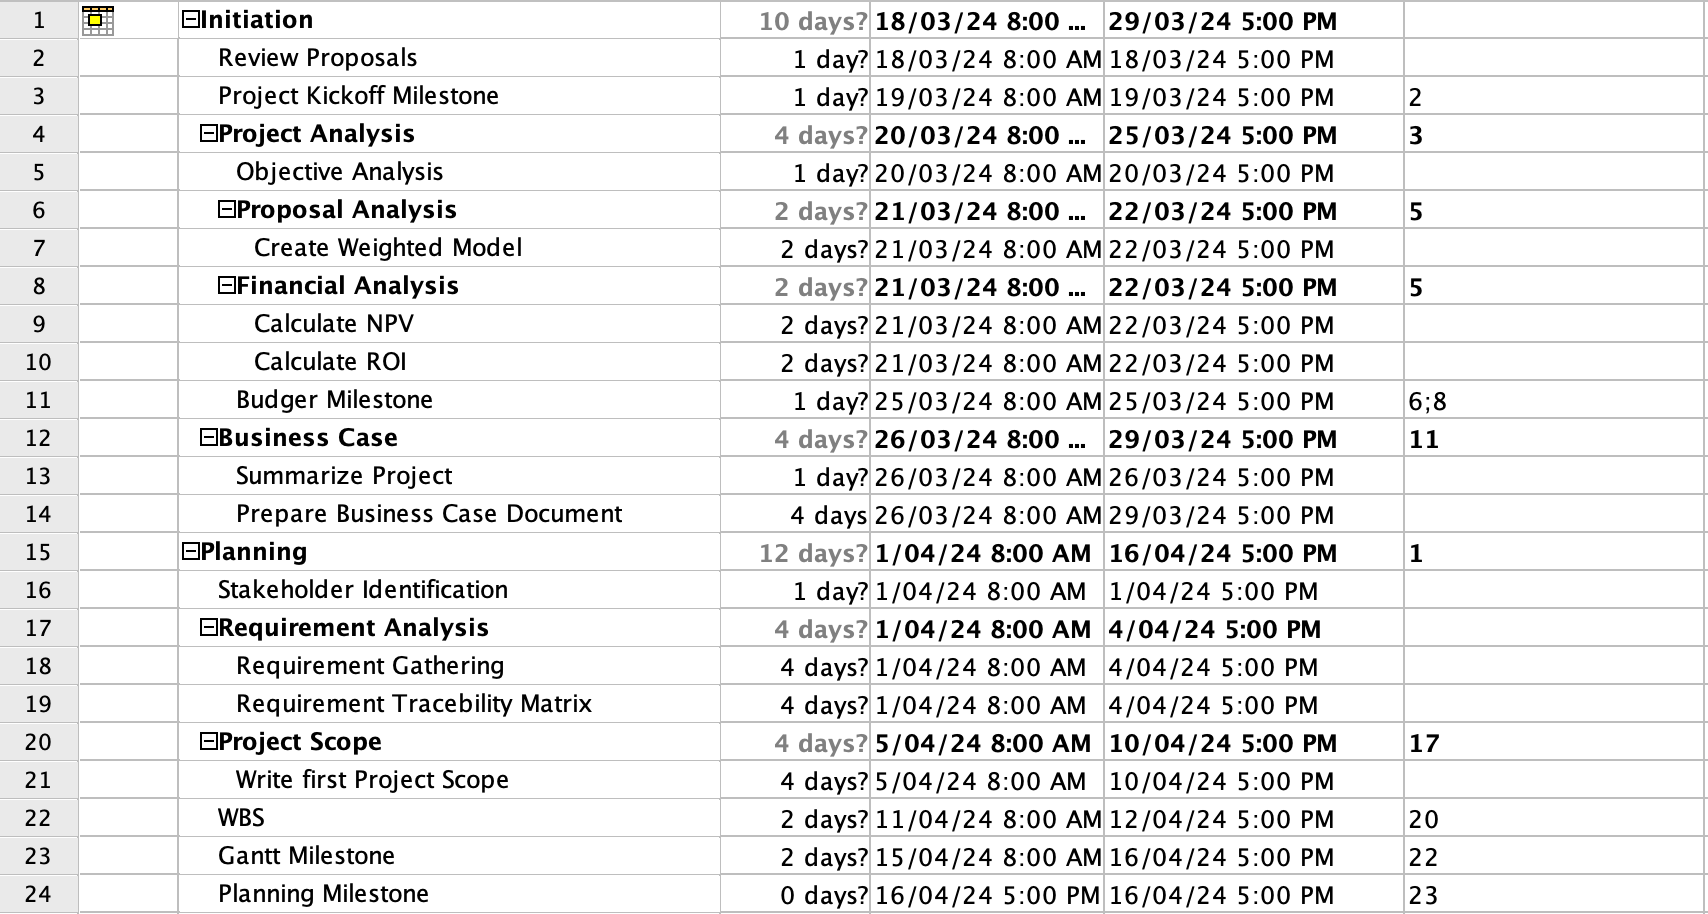
\includegraphics[width=\textwidth]{images/gantt_fill_1.png}
    \caption{Gantt Chart with Milestone 1}
    \label{fig:gnt3}
\end{figure}

\begin{figure}[ht]
    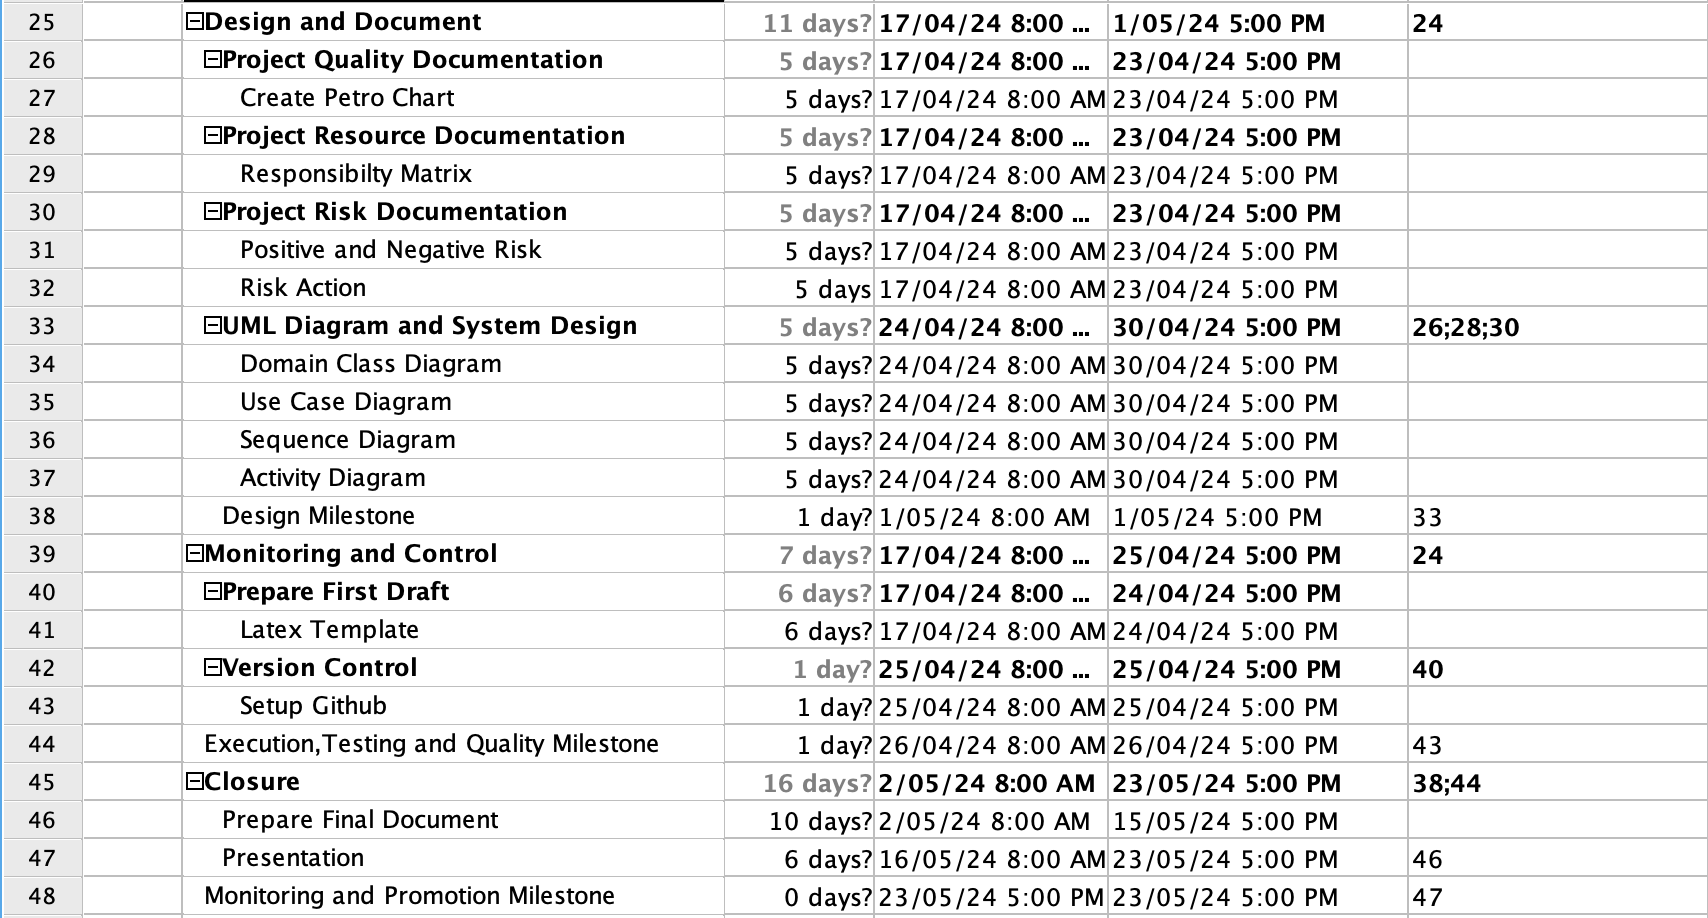
\includegraphics[width=\textwidth]{images/gantt_fill_2.png}
    \caption{Gantt Chart with Milestone 2}
    \label{fig:gnt4}
\end{figure}

\begin{figure}[ht]
    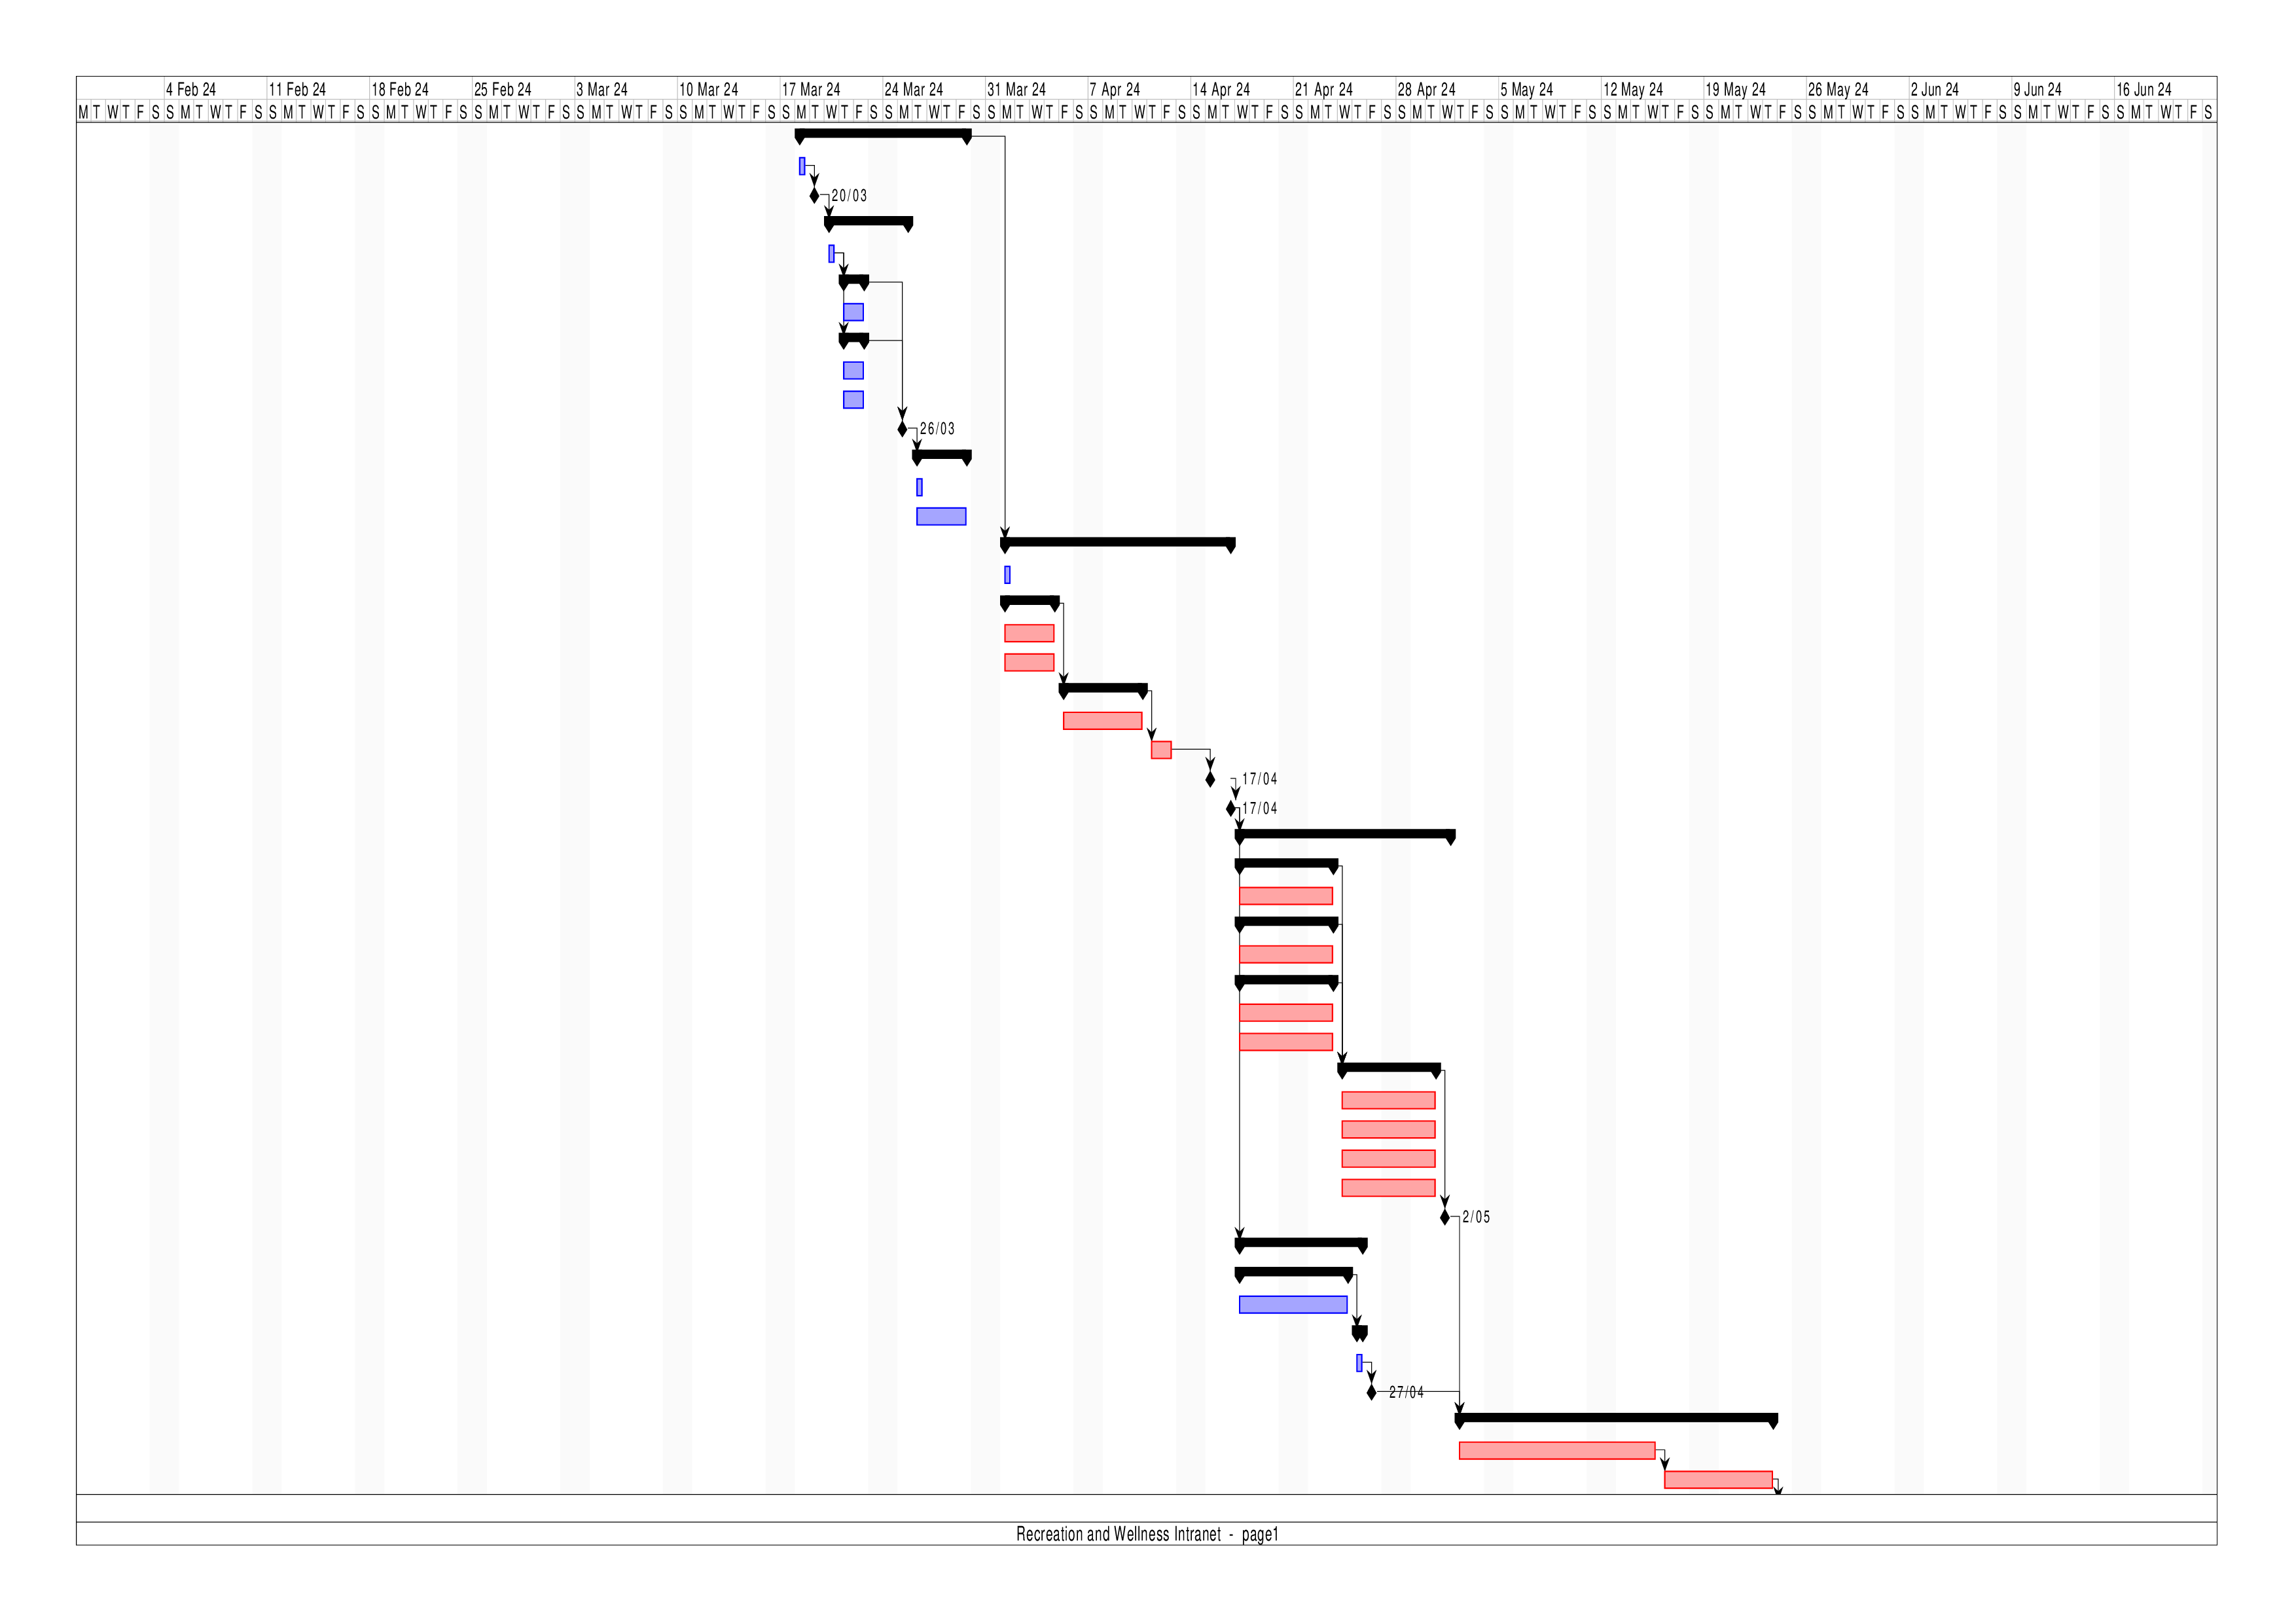
\includegraphics[width=\textwidth]{images/gantt_chart.png}
    \caption{Final Gantt Chart}
    \label{fig:gnt_chart}
\end{figure}

\begin{figure}[ht]
    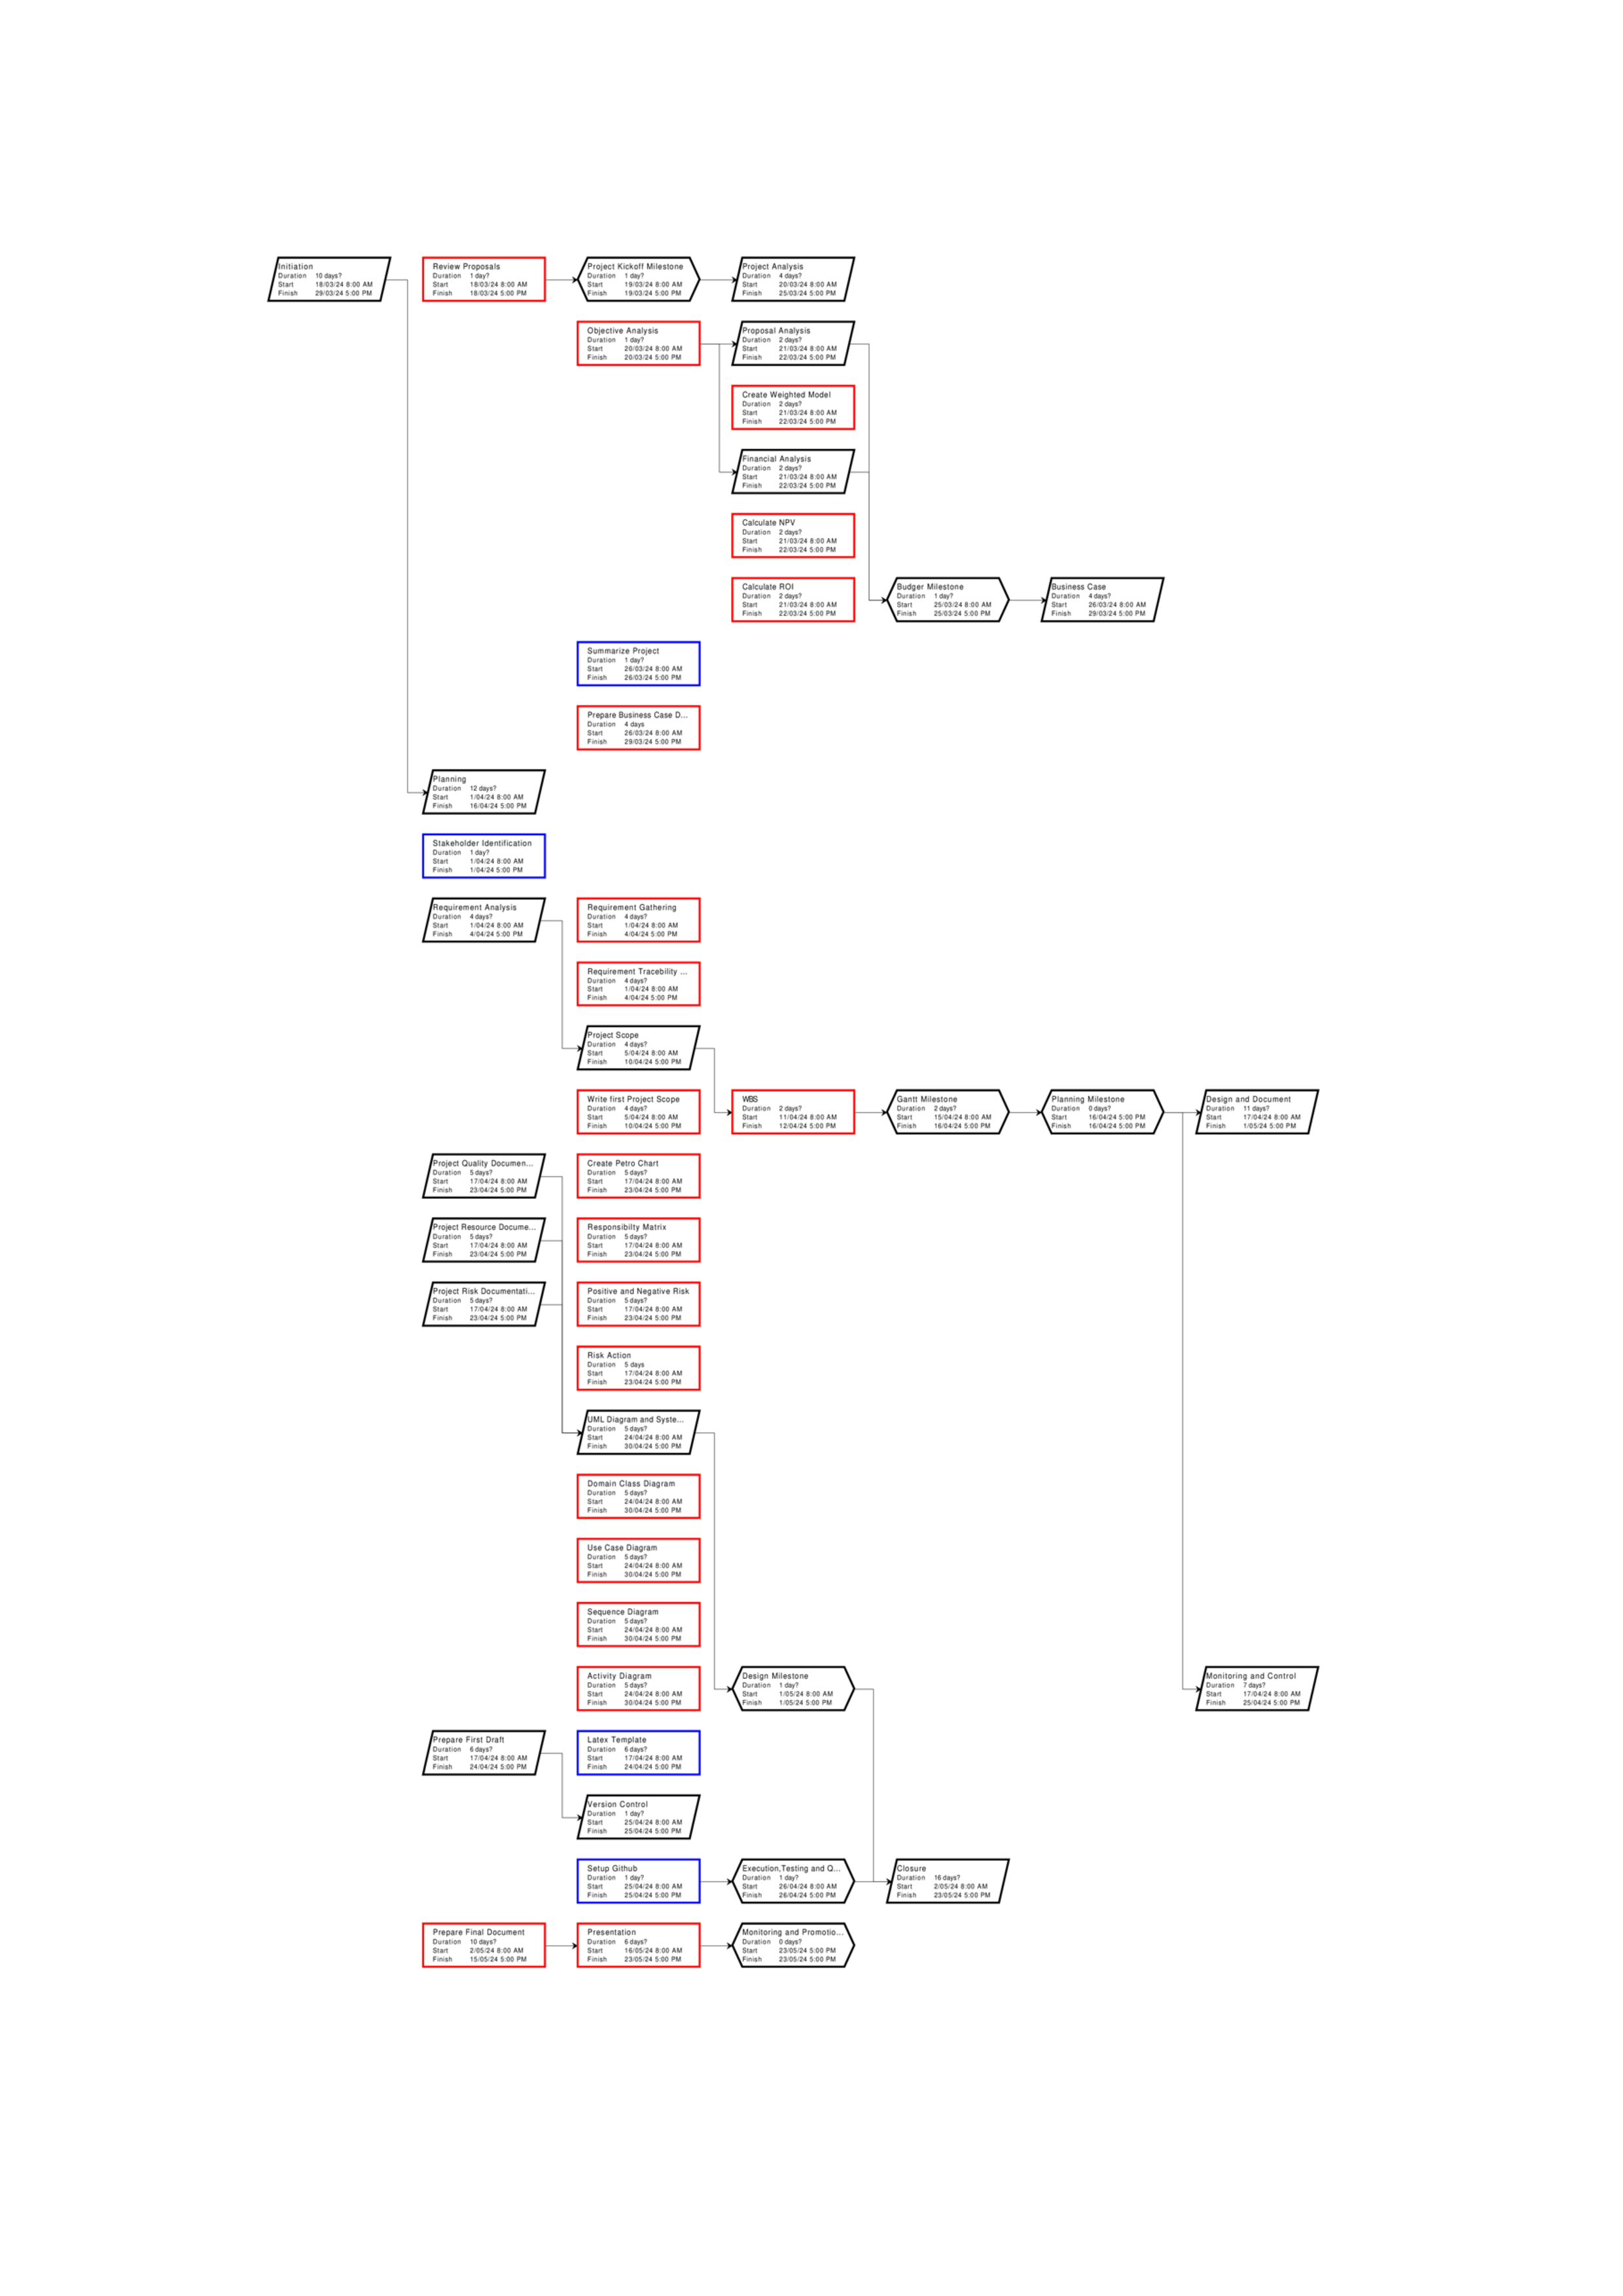
\includegraphics[width=\textwidth]{images/network.png}
    \caption{Network Diagram}
    \label{fig:rn_chart1}
\end{figure}

\FloatBarrier

\section{Milestone Report}

This section lists the status report on each milestone.

\subsection*{Late Milestones}
\begin{tabular}{|l|l|l|l|}
\hline
\rowcolor{lightred} Milestone Name & Expected Date & Finish Date & Delayed by \\
\hline
Execution Phase Completion Milestone & Fri 26/04/24 & Wed 08/05/24 & 13 days \\
\hline
Testing and Quality Assurance Milestone & Fri 26/04/24 & Wed 08/05/24 & 13 days \\
\hline
Design Phase Completion Milestone & Wed 01/05/24 & Wed 08/05/24 & 7 days \\
\hline
\end{tabular}

\subsection*{Milestones Due This Month}
\begin{tabular}{|l|l|}
\hline
\rowcolor{lightblue} Milestone Name & Finish Date \\
\hline
Monitoring and Promotion Milestone & Thu 23/05/24 \\
\hline
\end{tabular}

\subsection*{Completed Milestones}
\begin{tabular}{|l|l|}
\hline
\rowcolor{lightgreen} Milestone Name & Finish Date \\
\hline
Project Kick-Off Milestone & Tue 19/03/24 \\
\hline
Budget Approval Milestone & Mon 25/03/24 \\
\hline
Gantt Chart Creation Milestone & Tue 16/04/24 \\
\hline
Planning Phase Completion Milestone & Tue 16/04/24 \\
\hline
Execution Phase Completion Milestone & Wed 08/05/24 \\
\hline
Testing and Quality Assurance Milestone & Wed 08/05/24 \\
\hline
Design Phase Completion Milestone & Wed 08/05/24 \\
\hline
Monitoring and Promotion Milestone & Thu 23/05/24 \\
\hline
\end{tabular}

\subsection*{Next Milestone}
\textbf{Monitoring and Promotion} (Thu 23/05/24)

\subsection*{Milestone Graph}

\begin{figure}[ht]
    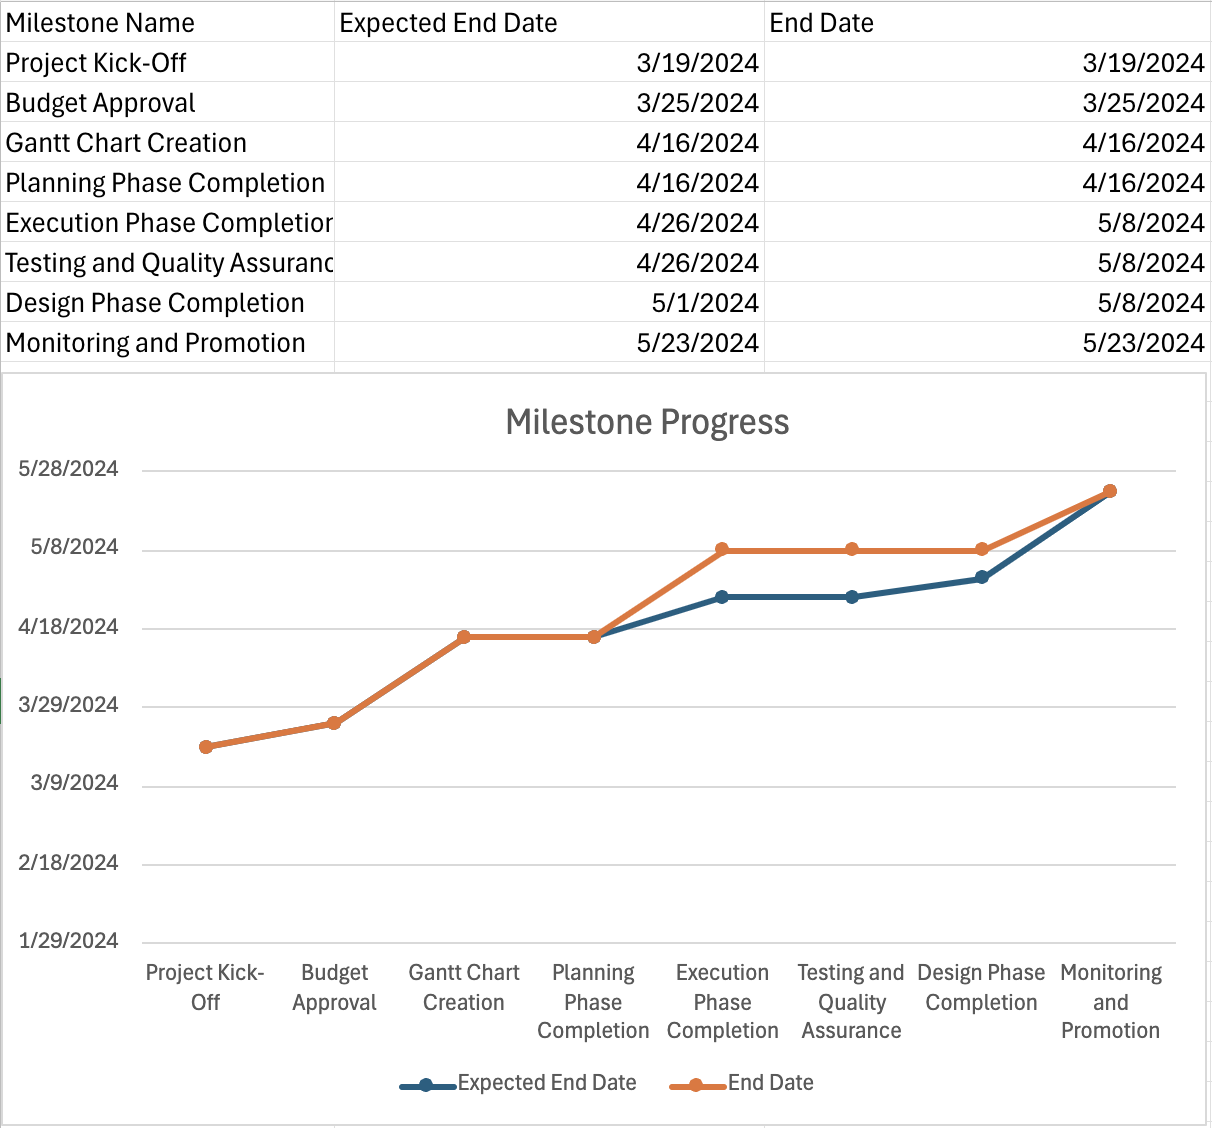
\includegraphics[width=\textwidth]{images/milestone-report.png}
    \caption{Milestone Progress Report}
    \label{fig:milestone_report}
\end{figure}


\FloatBarrier
\newpage